\subsection{Docker}
ในการศึกษาเรื่อง Docker \cite{docker} นั้นผมเลยที่จะใช้ Docker Desktop ในการศึกษาและเรียนรู้ใช้งาน
ดังนั้นในเอกสารนี้จะอ้างอิงการติดตั้ง Docker Desktop เป็นหลัก ทั้งนี้หากสนใจการใช้งานในรูปแบบอื่นสามารถเรียนรู้ได้จากเว็บไซต์ของ Docker ได้ที่ \url{https://docs.docker.com/get-docker/}
\subsubsection{วิธีติดตั้ง Docker Desktop}
\begin{enumerate}
      \item \textbf{ดาวน์โหลด Docker Desktop:}
            \begin{itemize}
                  \item ไปที่เว็บไซต์ \url{https://www.docker.com/products/docker-desktop}
                  \item เลือกเวอร์ชันที่ตรงกับระบบปฏิบัติการของคุณ (Windows หรือ macOS) แล้วคลิกดาวน์โหลด
            \end{itemize}

      \item \textbf{ติดตั้ง Docker Desktop:}
            \begin{itemize}
                  \item สำหรับ Windows:
                        \begin{enumerate}
                              \item เปิดไฟล์ติดตั้งที่ดาวน์โหลดมา (.exe)
                              \item ทำตามขั้นตอนในตัวช่วยติดตั้ง (Installer Wizard) เพื่อทำการติดตั้ง
                        \end{enumerate}
                  \item สำหรับ macOS:
                        \begin{enumerate}
                              \item เปิดไฟล์ติดตั้งที่ดาวน์โหลดมา (.dmg)
                              \item ลากไอคอน Docker ไปยังโฟลเดอร์ Applications
                              \item เปิดแอป Docker จากโฟลเดอร์ Applications
                        \end{enumerate}
            \end{itemize}

      \item \textbf{ทดลองรันคอนเทนเนอร์:}
            \begin{itemize}
                  \item รันคำสั่งทดสอบ:
                        \begin{minted}[frame=single,breaklines]{bash}
    $ docker run -dp 80:80 yeasy/simple-web:latest
            \end{minted}
                  \item คำสั่งนี้จะดาวน์โหลดและรันคอนเทนเนอร์ทดสอบเพื่อยืนยันว่า Docker Desktop ได้ติดตั้งและทำงานได้อย่างถูกต้อง สามารถเข้าเว็บไซต์ \url{http://localhost} เพื่อดูผลลัพธ์
            \end{itemize}
\end{enumerate}
\begin{figure}[ht]
      \begin{center}
            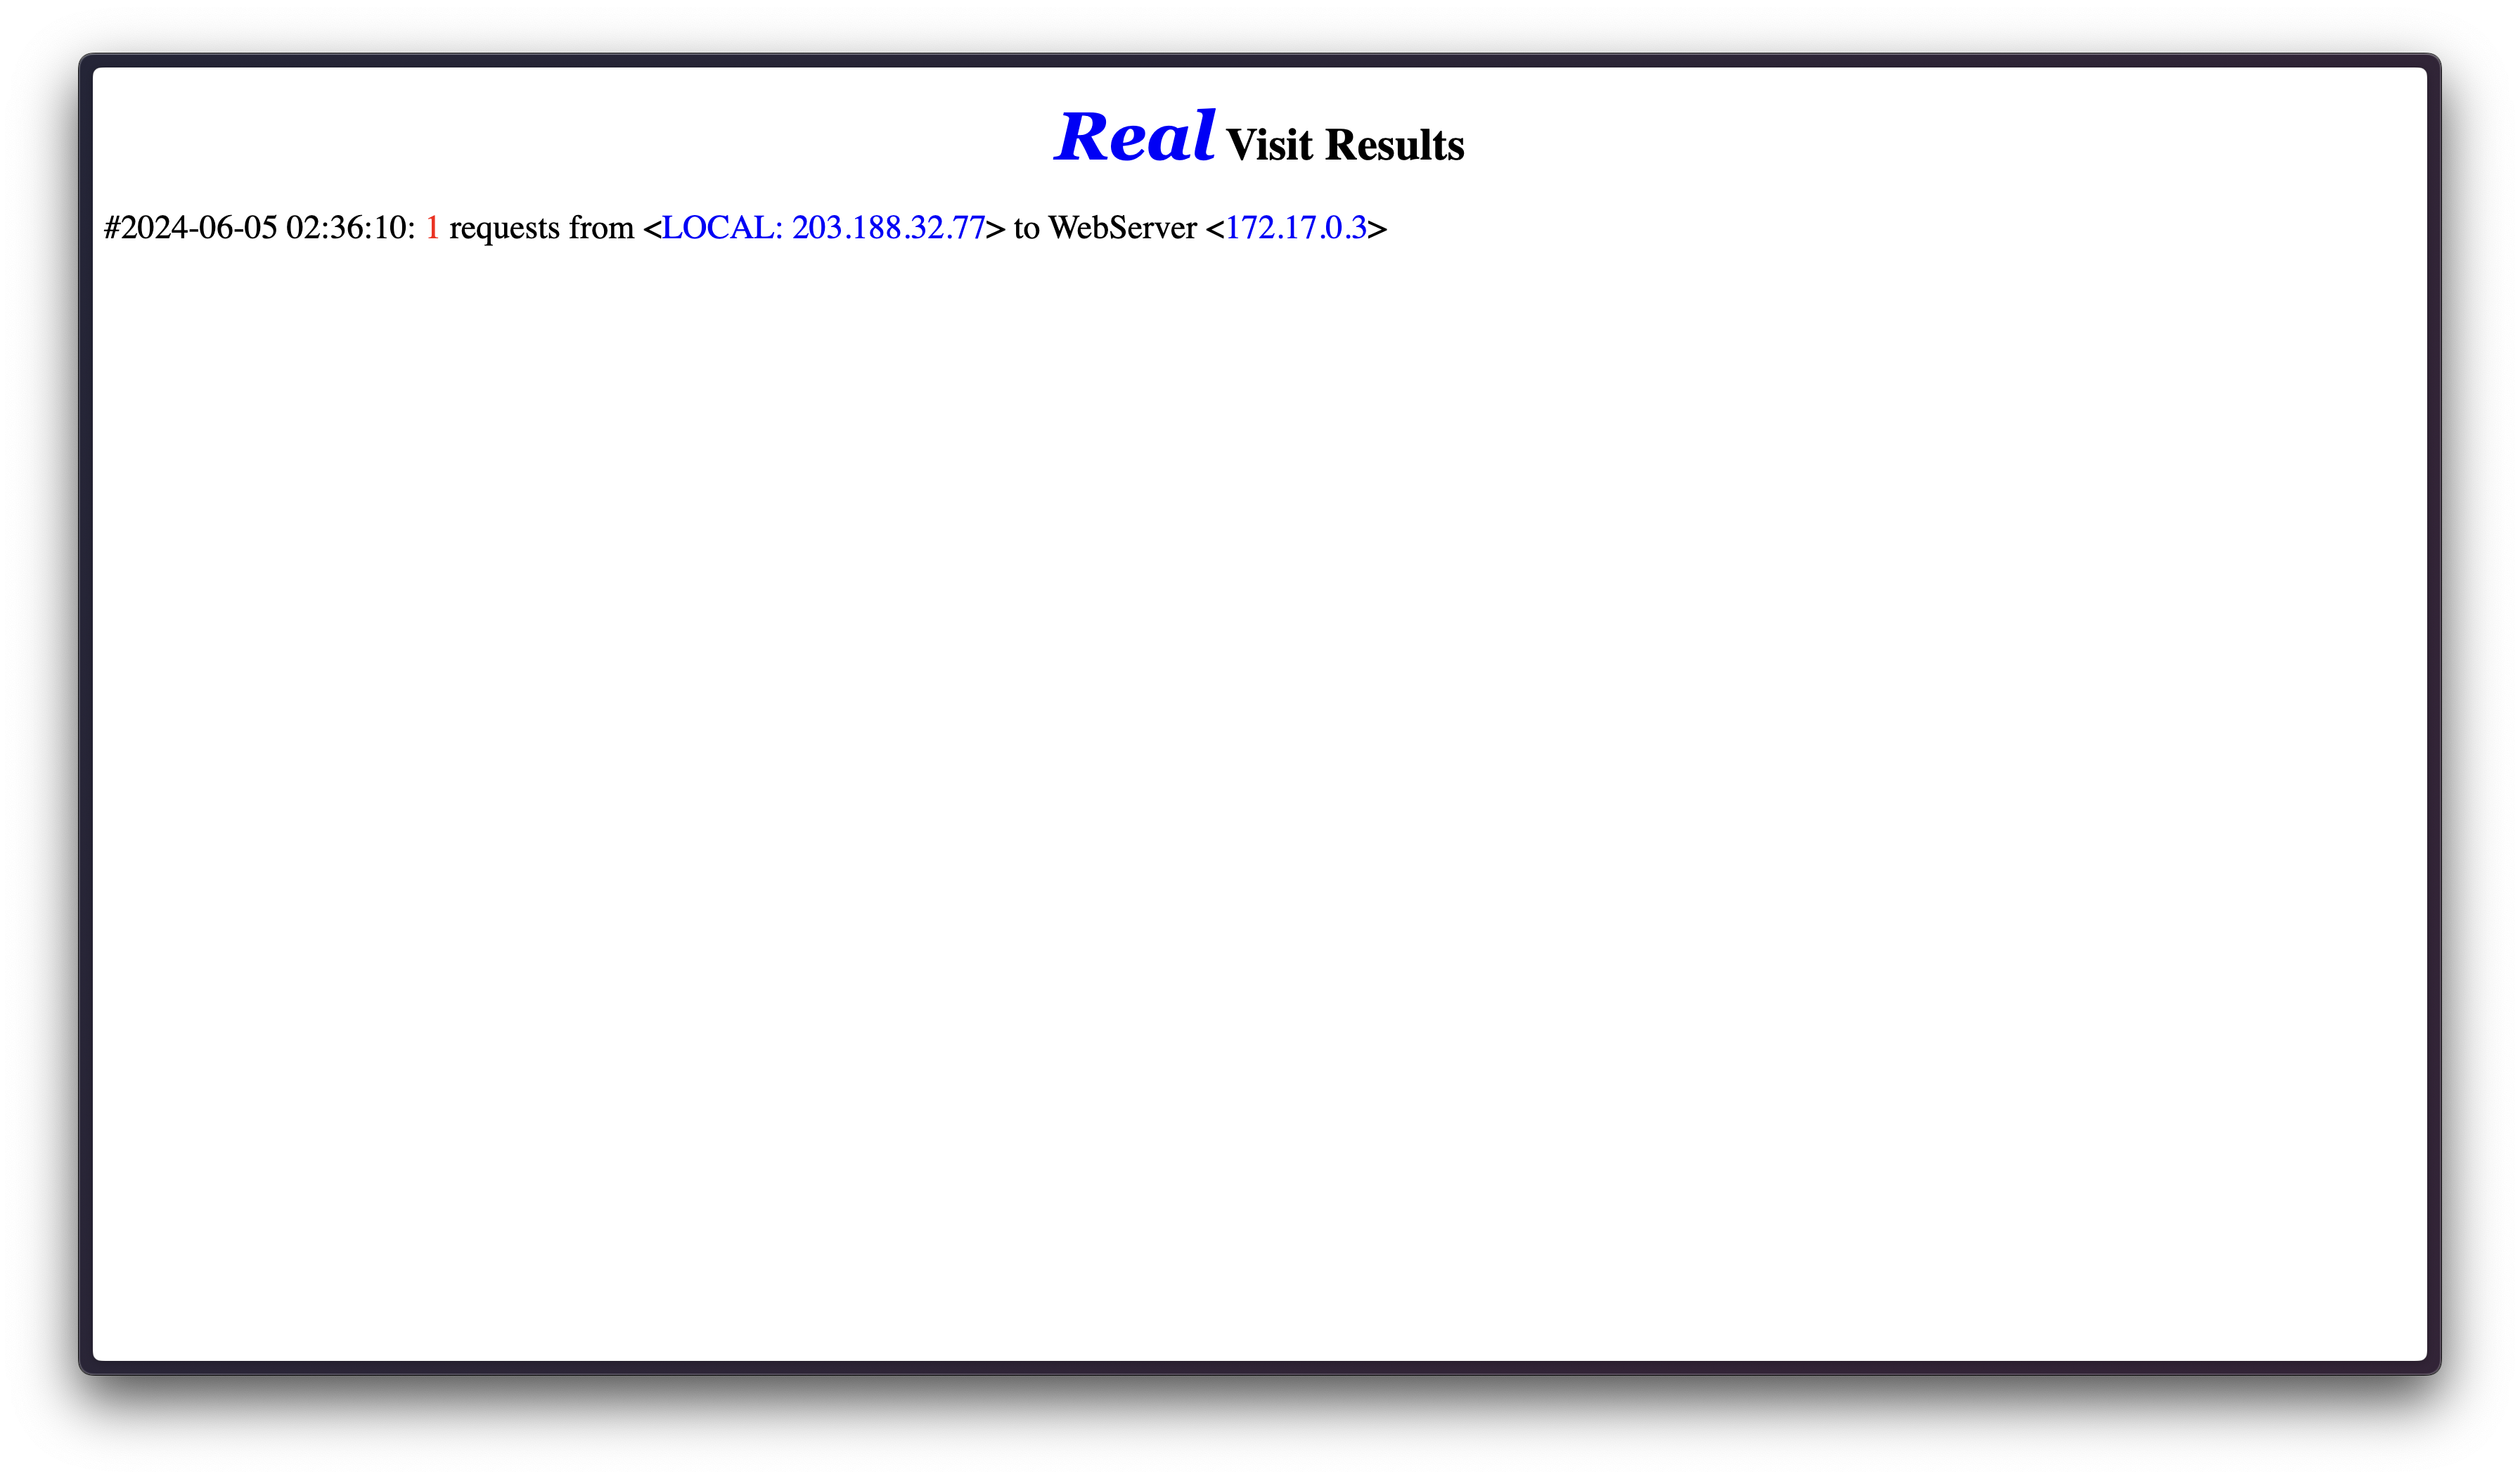
\includegraphics[scale=0.2]{images/simpleDockerRunResult.png}
      \end{center}
      \caption[ผลลัพธ์การรันคอนเทนเนอร์ทดสอบ]{ผลลัพธ์การรันคอนเทนเนอร์ทดสอบ}
\end{figure}

\clearpage
\subsubsection{วิธีสร้าง Docker Image}

เมื่อคุณพัฒนาแอปพลิเคชันของคุณแล้ว คุณจำเป็นต้องสร้าง Docker image สำหรับโปรเจ็กต์นั้นเพื่อให้สามารถรันบนคอนเทนเนอร์ได้ ในส่วนนี้เราจะแสดงวิธีง่าย ๆ ในการสร้าง Docker image ผ่าน Dockerfile และลองรันดู

\begin{enumerate}
      \item \textbf{สร้างแอปพลิเคชัน Node.js ตัวอย่าง:}
            \begin{enumerate}
                  \item สร้างโฟลเดอร์ว่างเพื่อเก็บ source code
                  \item รันคำสั่งต่อไปนี้:
                        \begin{minted}[frame=single,breaklines]{bash}
npm init -y  # สร้างโปรเจ็กต์ Node
npm i express  # ติดตั้งไลบรารี Express
        \end{minted}
                  \item เพิ่ม \mintinline{json}{"type": "module"} ลงในไฟล์ package.json ผลลัพธ์ควรจะเป็นดังนี้:
                        \begin{minted}[frame=single,breaklines]{json}
{
  "name": "simple-node-app",
  "version": "1.0.0",
  "main": "index.js",
  "type": "module",
  "scripts": {
    "test": "echo \"Error: no test specified\" && exit 1"
  },
  "keywords": [],
  "author": "",
  "license": "ISC",
  "description": "",
  "dependencies": {
    "express": "^4.19.2"
  }
}
        \end{minted}
                        \clearpage
                  \item สร้างไฟล์ index.js และเขียนโค้ดตัวอย่างดังนี้:
                        \begin{minted}[frame=single,breaklines]{javascript}
import express from "express";
import os from "os";

const app = express();
const port = 3000;

app.get("/", (req, res) => {
  res.send({
    message: `${os.hostname()} is running on port ${port}! with simple node js app`,
  });
});

app.listen(port, () => {
  console.log(`Server is running on port ${port}`);
});
        \end{minted}
                  \item ทดลองรันแอปด้วยคำสั่ง \mintinline{bash}{node index.js} จากนั้นเปิดเว็บเบราว์เซอร์และเข้าไปที่ \url{http://localhost:3000} ผลลัพธ์ควรจะแสดงข้อความจาก API
            \end{enumerate}

      \item \textbf{สร้าง Dockerfile:}
            \begin{enumerate}
                  \item สร้างไฟล์ชื่อ \texttt{Dockerfile} (ไม่มีนามสกุลไฟล์) ในโฟลเดอร์โปรเจ็กต์
                  \item เพิ่มเนื้อหาต่อไปนี้ลงในไฟล์ Dockerfile:
                        \begin{minted}[frame=single,breaklines]{dockerfile}
FROM node:14

WORKDIR /app

COPY package*.json ./

RUN npm install

COPY . .

EXPOSE 3000

CMD ["node", "index.js"]
        \end{minted}
            \end{enumerate}

      \item \textbf{สร้าง Docker Image:}
            \begin{enumerate}
                  \item เปิด Terminal และรันคำสั่งต่อไปนี้เพื่อสร้าง Docker image
                        \begin{minted}[frame=single,breaklines]{bash}
docker build -t my-node-app .
        \end{minted}
            \end{enumerate}

      \item \textbf{รัน Docker Container:}
            \begin{enumerate}
                  \item หลังจากสร้าง image เสร็จแล้ว รันคำสั่งต่อไปนี้เพื่อสร้างและรัน container:
                        \begin{minted}[frame=single,breaklines]{bash}
docker run -p 3000:3000 my-node-app
        \end{minted}
                  \item เปิดเว็บเบราว์เซอร์และเข้าไปที่ \url{http://localhost:3000} อีกครั้ง ควรจะเห็นผลลัพธ์เหมือนกับตอนรันแอปโดยตรง แต่ครั้งนี้แอปกำลังทำงานอยู่ใน Docker container
            \end{enumerate}
\end{enumerate}

\subsubsection{การ Push Image ไปยัง Registry}

\paragraph{Public Registry}
จากส่วนก่อนหน้านี้ เราได้สร้าง Docker image ชื่อ \texttt{simple-app} ในส่วนนี้เราจะ push มันไปยัง DockerHub ซึ่งเป็น public registry
ก่อนที่จะ push เราจำเป็นต้องสร้าง repository บน Docker Hub

\begin{enumerate}
      \item ให้ tag กับ simple-app ก่อนที่จะ push ไปยัง registry:
            \begin{minted}[frame=single,breaklines]{bash}
docker tag simple-app YOUR-USER-NAME/REPO_NAME
docker push YOUR-USER-NAME/REPO_NAME
    \end{minted}
      \item หากทุกอย่างทำงานได้อย่างถูกต้อง คุณจะเห็นผลลัพธ์การ push ขึ้นมา
\end{enumerate}

\paragraph{Private Registry}
สำหรับ private registry ขั้นตอนจะคล้ายกับ public repository แต่มีการเปลี่ยนแปลงบางอย่างในคำสั่งที่ใช้:

\begin{minted}[frame=single,breaklines]{bash}
docker tag [OPTIONS] IMAGE[:TAG] [REGISTRYHOST/][USERNAME/]NAME[:TAG]
docker push NAME[:TAG]
\end{minted}

\clearpage
\subsubsection{การรัน Container}

มีหลายวิธีในการรัน Docker container วิธีหนึ่งที่เราใช้ไปแล้วคือการใช้คำสั่ง \mintinline{bash}{docker run} อีกวิธีหนึ่งคือการเขียนไฟล์ \texttt{docker-compose} ในส่วนนี้เราจะสร้างไฟล์ docker-compose อย่างง่ายเพื่อรัน simple-app

\begin{enumerate}
      \item สร้างไฟล์ \texttt{docker-compose.yml} และเขียน YAML file ดังนี้:
            \begin{minted}[frame=single,breaklines]{yaml}
version: "3"
services:
  simple-app:
    image: IMAGETAG
    ports:
      - "80:3000"
    \end{minted}

      \item รัน container ด้วยคำสั่ง:
            \begin{minted}[frame=single,breaklines]{bash}
docker-compose up -d
    \end{minted}
            คำสั่งนี้จะรัน container ด้วย image simple-app
\end{enumerate}